\begin{exercice*}  
  Madame Martin souhaite réaliser une terrasse en béton en face de sa baie vitrée.\\\medskip
  Elle réalise le dessin ci-dessous.\\\smallskip    
  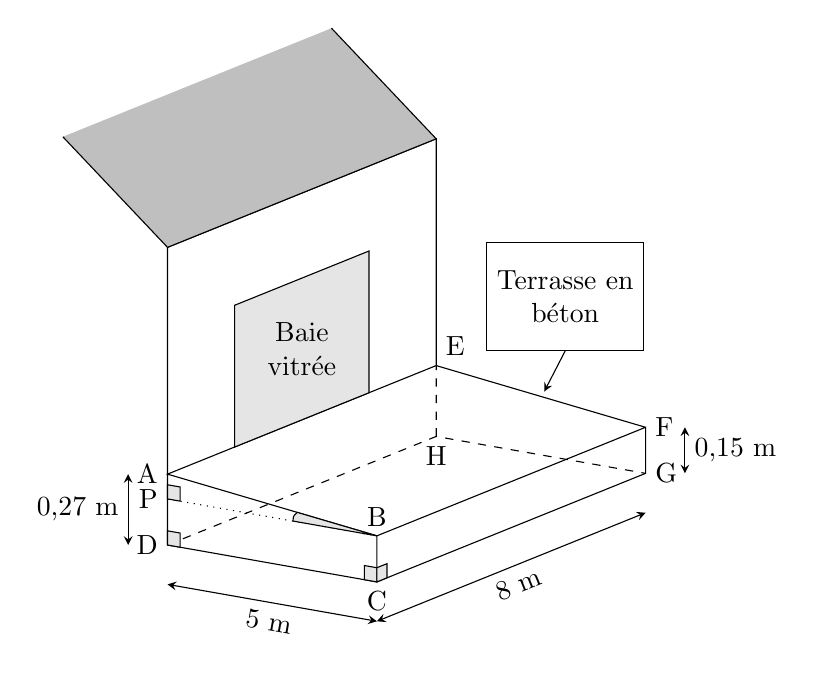
\begin{tikzpicture}[baseline = {(current bounding box.center)},x={(-158:0.46cm)},y = {(-10:0.54cm)},z = {(90:0.9cm)} ,> = stealth]
    \draw[dashed] (8,0,0) -- (0,0,0) -- (0,5,0) (0,0,0) -- (0,0,1);
    \draw (8,0,0) -- (8,5,0) -- (0,5,0) -- (0,5,0.65) -- (8,5,0.65) -- (8,0,1)--(0,0,1) -- (0,5,0.65) %terrasse
    (8,5,0)--(8,5,0.65) %coin de la terrasse
    (8,0,0) --(8,0,4.2) -- (0,0,4.2)--(0,0,1); %facade avant de la maison;
    \filldraw[fill = gray!50, draw=black] (0,-2.5,5.5) -- (0,0,4.2) -- (8,0,4.2) --(8,-2.5,5.5) ;%toit; 
    \filldraw[fill = gray!20, draw=black] (6,0,1) -- (6,0,3) --(2,0,3) --(2,0,1) -- cycle ;%baie vitrée;	
    \node at (4,0,2) {\parbox{1cm}{\begin{center} Baie vitrée \end{center}}};
    \draw [shift = {(-5mm,0mm)},<->] (8,0,0) -- (8,0,1) node [pos = 0.5, left] {0,27 m} ;
    \draw [shift = {(0mm,-5mm)},<->] (8,0,0) -- (8,5,0) node [pos = 0.5,sloped, below] {5 m} ;
    \draw [shift = {(0mm,-5mm)},<->] (8,5,0) -- (0,5,0) node [pos = 0.5, sloped, below ] {8 m} ;
    \draw [shift = {(5mm,0mm)},<->] (0,5,0) -- (0,5,0.65) node [pos = 0.5, right] {0,15 m} ;
    \draw[dotted] (8,0,0.65) -- (8,5,0.65);
    \filldraw[fill = gray!20, draw=black,shift = {(8,0,0)}]  (0,0,0) -- (0,0.3,0) --(0,0.3,0.2) --(0,0,0.2) -- cycle ;%angle droit;
    \filldraw[fill = gray!20, draw=black,shift = {(8,0,0.65)}] (0,0,0) -- (0,0.3,0) --(0,0.3,0.2) --(0,0,0.2) -- cycle ;%angle droit;
    \filldraw[fill = gray!20, draw=black,shift = {(8,4.7,0)}] (0,0,0) -- (0,0.3,0) --(0,0.3,0.2) --(0,0,0.2) -- cycle ;%angle droit;		
    \filldraw[fill = gray!20, draw=black,shift = {(8,5,0)}] (0,0,0) -- (-0.3,0,0) --(-0.3,0,0.2) --(0,0,0.2) -- cycle ;%angle droit;
    \draw[<-] (-0.10,2.5,0.875) -- (-0.10,3,1.5) node [above,draw,inner sep=0]{\parbox{2cm}{\begin{center} Terrasse en béton \end{center}}};
    \node at (8,0,1) [left] {A};
    \node at (8,5,0.65) [above] {B};
    \node at (8,5,0) [below] {C};
    \node at (8,0,0) [left] {D};
    \node at (0,0,1) [above right] {E};
    \node at (0,5,0.65) [right] {F};
    \node at (0,5,0) [right] {G};
    \node at (0,0,0) [below] {H};
    \node at (8,0,0.65) [left] {P};
    \filldraw [fill = gray!20, draw=black] (8,5,0.65) -- (8,3.,0.65) .. controls (8,3,0.72) .. (8,3.1,0.783) -- cycle;
  \end{tikzpicture}
  
  Pour faciliter l'écoulement des eaux de pluie, le sol de la terrasse doit être incliné.\\\smallskip
  La terrasse a la forme d'un prisme droit dont la base est le quadrilatère ABCD et la hauteur est le segment [CG].\\\smallskip    
  P est le point du segment [AD] tel que BCDP est un rectangle\\.
  L'angle $ \widehat{\text{ABP}} $ doit mesurer entre 1° et 1,5°.
  Le projet de Madame Martin vérifie-t-il cette condition ?
\end{exercice*}
% \begin{corrige}
%   %\setcounter{partie}{0} % Pour s'assurer que le compteur de \partie est à zéro dans les corrigés
%   % \phantom{rrr}    
%   \dots
% \end{corrige}